% Options for packages loaded elsewhere
\PassOptionsToPackage{unicode}{hyperref}
\PassOptionsToPackage{hyphens}{url}
\documentclass[
]{article}
\usepackage{xcolor}
\usepackage[margin=1in]{geometry}
\usepackage{amsmath,amssymb}
\setcounter{secnumdepth}{5}
\usepackage{iftex}
\ifPDFTeX
  \usepackage[T1]{fontenc}
  \usepackage[utf8]{inputenc}
  \usepackage{textcomp} % provide euro and other symbols
\else % if luatex or xetex
  \usepackage{unicode-math} % this also loads fontspec
  \defaultfontfeatures{Scale=MatchLowercase}
  \defaultfontfeatures[\rmfamily]{Ligatures=TeX,Scale=1}
\fi
\usepackage{lmodern}
\ifPDFTeX\else
  % xetex/luatex font selection
\fi
% Use upquote if available, for straight quotes in verbatim environments
\IfFileExists{upquote.sty}{\usepackage{upquote}}{}
\IfFileExists{microtype.sty}{% use microtype if available
  \usepackage[]{microtype}
  \UseMicrotypeSet[protrusion]{basicmath} % disable protrusion for tt fonts
}{}
\makeatletter
\@ifundefined{KOMAClassName}{% if non-KOMA class
  \IfFileExists{parskip.sty}{%
    \usepackage{parskip}
  }{% else
    \setlength{\parindent}{0pt}
    \setlength{\parskip}{6pt plus 2pt minus 1pt}}
}{% if KOMA class
  \KOMAoptions{parskip=half}}
\makeatother
\usepackage{longtable,booktabs,array}
\usepackage{calc} % for calculating minipage widths
% Correct order of tables after \paragraph or \subparagraph
\usepackage{etoolbox}
\makeatletter
\patchcmd\longtable{\par}{\if@noskipsec\mbox{}\fi\par}{}{}
\makeatother
% Allow footnotes in longtable head/foot
\IfFileExists{footnotehyper.sty}{\usepackage{footnotehyper}}{\usepackage{footnote}}
\makesavenoteenv{longtable}
\usepackage{graphicx}
\makeatletter
\newsavebox\pandoc@box
\newcommand*\pandocbounded[1]{% scales image to fit in text height/width
  \sbox\pandoc@box{#1}%
  \Gscale@div\@tempa{\textheight}{\dimexpr\ht\pandoc@box+\dp\pandoc@box\relax}%
  \Gscale@div\@tempb{\linewidth}{\wd\pandoc@box}%
  \ifdim\@tempb\p@<\@tempa\p@\let\@tempa\@tempb\fi% select the smaller of both
  \ifdim\@tempa\p@<\p@\scalebox{\@tempa}{\usebox\pandoc@box}%
  \else\usebox{\pandoc@box}%
  \fi%
}
% Set default figure placement to htbp
\def\fps@figure{htbp}
\makeatother
\setlength{\emergencystretch}{3em} % prevent overfull lines
\providecommand{\tightlist}{%
  \setlength{\itemsep}{0pt}\setlength{\parskip}{0pt}}
\usepackage{bookmark}
\IfFileExists{xurl.sty}{\usepackage{xurl}}{} % add URL line breaks if available
\urlstyle{same}
\hypersetup{
  pdftitle={INFO248-project2ms1-Wong-Wu},
  pdfauthor={Zijian Wu \& Adrian Wong},
  hidelinks,
  pdfcreator={LaTeX via pandoc}}

\title{INFO248-project2ms1-Wong-Wu}
\author{Zijian Wu \& Adrian Wong}
\date{04/03/2026}

\begin{document}
\maketitle

\section{Overview}\label{overview}

There are many factors that determine the salary of a job. There are
aspects that the job requires and qualities that the applicant can
uniquely bring. Knowing how each of these predictors affect the salary
of a job is of major interest to employers and those looking to be
employed as they help them gauge the market.

The main research question of this analysis is how do personal and job
factors contribute to a the predicted salary of a job?

\section{Data Description and
Processing}\label{data-description-and-processing}

The dataset used in this analysis was come from Kaggle{[}1{]}. We
categorized the variables in the dataset as personal and job based.
Knowing how these different factors affect possible job salaries is of
major interest to both employers and applicants to gauge the market.

Personal Variables:\\
Experience years:Number of years of professional experience. Numeric\\
Education level:Highest level of education completed. Categorical\\
Skills count: Number of technical or professional skills. Numeric\\
Certifications: Number of professional certifications. Numeric\\

Job Variables:\\
Job title: The job role or position (e.g.Data Analyst, AI engineer).
Categorical\\
Industry: Industry sector where the job belongs. Categorical\\
Company size: Size of the company (small, medium, large). Categorical\\
Location: Job location or region. Categorical\\
Remote Work:Whether the job allows remote work. Categorical\\

Outcome Variable: Salary: Annual salary of the employee. Numeric\\

The dataset was check for missing values. Of the original 250,000
observations, we found 0 observation that contained missing value.

\section{Data Exploration}\label{data-exploration}

In figure 1, the distribution of the outcome variable, salary, shows a
mostly symmetrical shape that is mildly skewed to the right.

\begin{figure}

{\centering 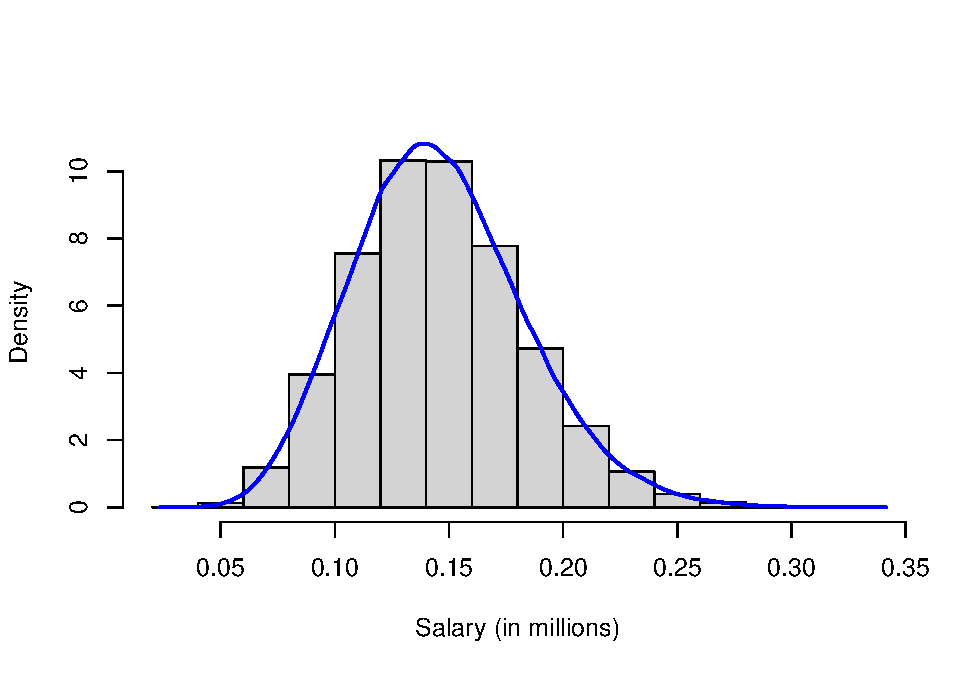
\includegraphics[width=0.65\linewidth,height=0.28\textheight]{INFO248-project2ms1-Wong-Wu_files/figure-latex/unnamed-chunk-3-1} 

}

\caption{Salary Density}\label{fig:unnamed-chunk-3}
\end{figure}

Since the median is lower than the mean, the data is slightly
right-skewed.

\begin{longtable}[]{@{}ll@{}}
\caption{Salary descriptive statistics}\tabularnewline
\toprule\noalign{}
statistic & value \\
\midrule\noalign{}
\endfirsthead
\toprule\noalign{}
statistic & value \\
\midrule\noalign{}
\endhead
\bottomrule\noalign{}
\endlastfoot
Min & 31867 \\
Mean & 145718.08 \\
Median & 143453 \\
Max & 333046 \\
StdDev & 37407.95 \\
\end{longtable}

The distribution of the histogram is a uniform distribution with a
non-obvious outlier at the low end

\begin{figure}

{\centering 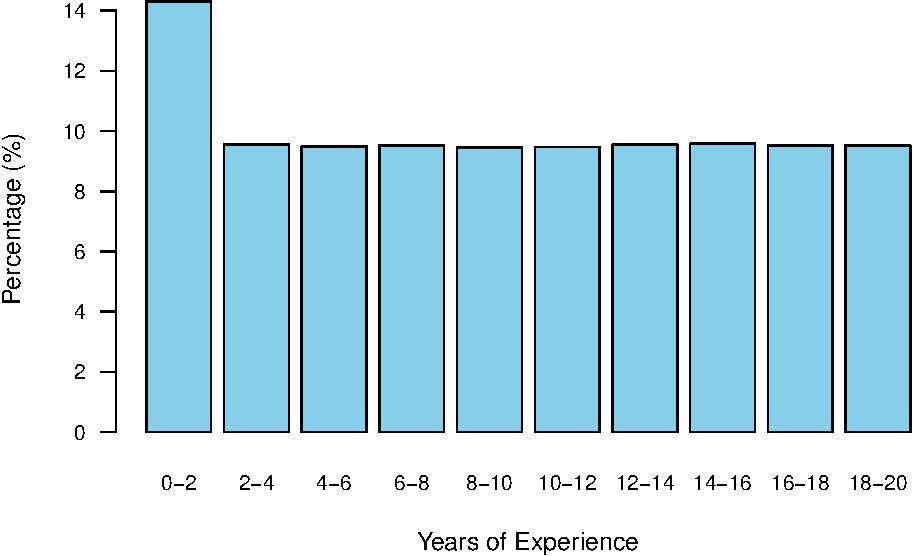
\includegraphics[width=0.65\linewidth,height=0.28\textheight]{INFO248-project2ms1-Wong-Wu_files/figure-latex/unnamed-chunk-5-1} 

}

\caption{Years of Experience and Percentage}\label{fig:unnamed-chunk-5}
\end{figure}

\newpage

The table below illustrates the frequency and percentage of each year of
experience.

\begin{longtable}[]{@{}lrr@{}}
\caption{Years of Experience, Frequency, and Percentage.}\tabularnewline
\toprule\noalign{}
Range of Experience & Frequency & Percentage (\%) \\
\midrule\noalign{}
\endfirsthead
\toprule\noalign{}
Range of Experience & Frequency & Percentage (\%) \\
\midrule\noalign{}
\endhead
\bottomrule\noalign{}
\endlastfoot
{[}0,2{]} & 35765 & 14.31 \\
(2,4{]} & 23891 & 9.56 \\
(4,6{]} & 23722 & 9.49 \\
(6,8{]} & 23803 & 9.52 \\
(8,10{]} & 23633 & 9.45 \\
(10,12{]} & 23691 & 9.48 \\
(12,14{]} & 23865 & 9.55 \\
(14,16{]} & 23960 & 9.58 \\
(16,18{]} & 23837 & 9.53 \\
(18,20{]} & 23833 & 9.53 \\
\end{longtable}

According to the data, the mean salary for entry-level positions is
approximately \$30,000 less than that of experienced roles. This
observation is based solely on years of experience and does not account
for variables such as job title

\begin{longtable}[]{@{}lr@{}}
\caption{Salary Comparison: Entry Level vs.~Experienced}\tabularnewline
\toprule\noalign{}
Experience Group & Mean Salary \\
\midrule\noalign{}
\endfirsthead
\toprule\noalign{}
Experience Group & Mean Salary \\
\midrule\noalign{}
\endhead
\bottomrule\noalign{}
\endlastfoot
Entry Level (0 Years) & 118,872.6 \\
Experienced (1+ Years) & 147,048.4 \\
\end{longtable}

The line plot demonstrates a positive correlation between years of
experience and salary. This upward trend indicates that as professional
experience increases, compensation levels tend to rise accordingly

\begin{figure}

{\centering 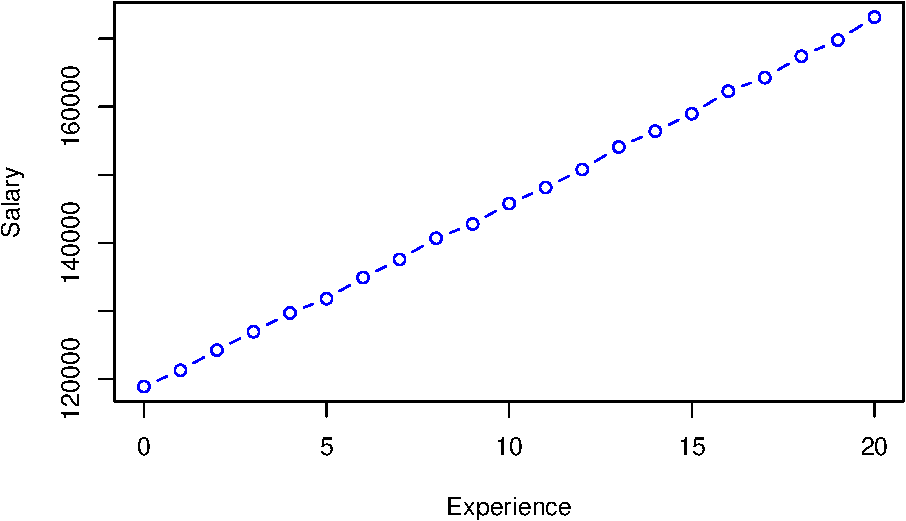
\includegraphics[width=0.65\linewidth,height=0.28\textheight]{INFO248-project2ms1-Wong-Wu_files/figure-latex/unnamed-chunk-8-1} 

}

\caption{Average salary by years of experience.}\label{fig:unnamed-chunk-8}
\end{figure}

\newpage

The distribution of the Job Title is uniform distributed, nearly all of
the job title has the similar percentage.

\begin{figure}

{\centering 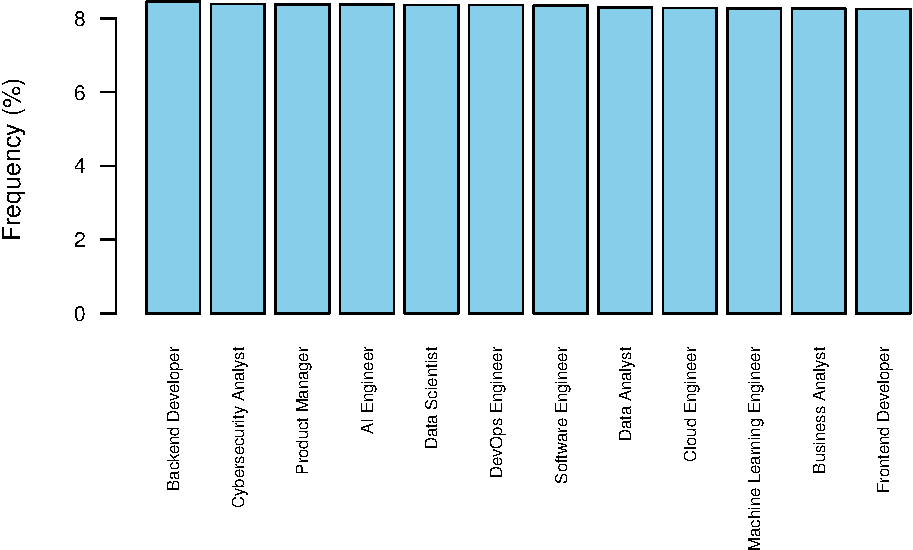
\includegraphics{INFO248-project2ms1-Wong-Wu_files/figure-latex/unnamed-chunk-9-1} 

}

\caption{Job Title Distribution}\label{fig:unnamed-chunk-9}
\end{figure}

Due to the uniform distribution of the data, the frequency and
percentage for each category are nearly equal, with every job
representing a consistent share of approximately 8\%

\begin{longtable}[]{@{}llrr@{}}
\caption{Job title frequency and percentage.}\tabularnewline
\toprule\noalign{}
& Job Title & Frequency & Percentage (\%) \\
\midrule\noalign{}
\endfirsthead
\toprule\noalign{}
& Job Title & Frequency & Percentage (\%) \\
\midrule\noalign{}
\endhead
\bottomrule\noalign{}
\endlastfoot
2 & Backend Developer & 21125 & 8.45 \\
5 & Cybersecurity Analyst & 20959 & 8.38 \\
11 & Product Manager & 20950 & 8.38 \\
1 & AI Engineer & 20945 & 8.38 \\
7 & Data Scientist & 20890 & 8.36 \\
8 & DevOps Engineer & 20889 & 8.36 \\
12 & Software Engineer & 20876 & 8.35 \\
6 & Data Analyst & 20722 & 8.29 \\
4 & Cloud Engineer & 20686 & 8.27 \\
10 & Machine Learning Engineer & 20677 & 8.27 \\
3 & Business Analyst & 20648 & 8.26 \\
9 & Frontend Developer & 20633 & 8.25 \\
\end{longtable}

\newpage

\section{Modeling}\label{modeling}

We fitted a target encoded linear regression model and random forest on
all of the factors that contribute to a job's salary.

\subsection{Hypothesis}\label{hypothesis}

We hypothesize that job-based factors, specifically job title and
location, will be stronger predictors of salary than personal factors
such as experience years and education level.

\subsection{Model 1}\label{model-1}

We fitted a linear regression model using all the predictors, with
salary as the predicted variable.The estimates for the coefficients,
standard errors and significance results are displayed below:

\begin{longtable}[]{@{}
  >{\raggedright\arraybackslash}p{(\linewidth - 8\tabcolsep) * \real{0.3375}}
  >{\raggedleft\arraybackslash}p{(\linewidth - 8\tabcolsep) * \real{0.1625}}
  >{\raggedleft\arraybackslash}p{(\linewidth - 8\tabcolsep) * \real{0.1375}}
  >{\raggedleft\arraybackslash}p{(\linewidth - 8\tabcolsep) * \real{0.1250}}
  >{\raggedleft\arraybackslash}p{(\linewidth - 8\tabcolsep) * \real{0.2375}}@{}}
\caption{Model 1 coefficient estimates, standard errors, and
significance.}\tabularnewline
\toprule\noalign{}
\begin{minipage}[b]{\linewidth}\raggedright
\end{minipage} & \begin{minipage}[b]{\linewidth}\raggedleft
Estimate
\end{minipage} & \begin{minipage}[b]{\linewidth}\raggedleft
Std. Error
\end{minipage} & \begin{minipage}[b]{\linewidth}\raggedleft
t value
\end{minipage} & \begin{minipage}[b]{\linewidth}\raggedleft
Pr(\textgreater\textbar t\textbar)
\end{minipage} \\
\midrule\noalign{}
\endfirsthead
\toprule\noalign{}
\begin{minipage}[b]{\linewidth}\raggedright
\end{minipage} & \begin{minipage}[b]{\linewidth}\raggedleft
Estimate
\end{minipage} & \begin{minipage}[b]{\linewidth}\raggedleft
Std. Error
\end{minipage} & \begin{minipage}[b]{\linewidth}\raggedleft
t value
\end{minipage} & \begin{minipage}[b]{\linewidth}\raggedleft
Pr(\textgreater\textbar t\textbar)
\end{minipage} \\
\midrule\noalign{}
\endhead
\bottomrule\noalign{}
\endlastfoot
(Intercept) & -181568.9293 & 10163.4909 & -17.8648 & 0.0000 \\
job\_title & 1.0051 & 0.0011 & 910.1622 & 0.0000 \\
experience\_years & 2698.0305 & 2.7347 & 986.5844 & 0.0000 \\
education\_levelDiploma & -5287.5279 & 52.4709 & -100.7707 & 0.0000 \\
education\_levelHigh School & -10664.3465 & 52.3504 & -203.7109 &
0.0000 \\
education\_levelMaster & 10806.0616 & 52.3739 & 206.3253 & 0.0000 \\
education\_levelPhD & 21581.1334 & 52.4248 & 411.6590 & 0.0000 \\
skills\_count & 860.1076 & 3.0252 & 284.3106 & 0.0000 \\
industry & 0.1010 & 0.0697 & 1.4489 & 0.1474 \\
company\_sizeLarge & -14131.9346 & 52.3400 & -270.0026 & 0.0000 \\
company\_sizeMedium & -28311.9427 & 52.4276 & -540.0199 & 0.0000 \\
company\_sizeSmall & -35399.1260 & 52.3692 & -675.9529 & 0.0000 \\
company\_sizeStartup & -42390.3793 & 52.5406 & -806.8115 & 0.0000 \\
location & 0.9980 & 0.0008 & 1285.8028 & 0.0000 \\
remote\_workNo & 19.3789 & 40.5606 & 0.4778 & 0.6328 \\
remote\_workYes & 5351.1399 & 40.6116 & 131.7638 & 0.0000 \\
certifications & 1614.6015 & 9.7118 & 166.2516 & 0.0000 \\
\end{longtable}

The adjusted R-squared for this model was 0.9633, meaning the model
explains approximately 96.3\% of the variance in salary.

\begin{longtable}[]{@{}lrrrl@{}}
\caption{Overall F-test results for Model 1.}\tabularnewline
\toprule\noalign{}
& F Statistic & Numerator df & Denominator df & p-value \\
\midrule\noalign{}
\endfirsthead
\toprule\noalign{}
& F Statistic & Numerator df & Denominator df & p-value \\
\midrule\noalign{}
\endhead
\bottomrule\noalign{}
\endlastfoot
value & 307507.1 & 16 & 187481 & 0e+00 \\
\end{longtable}

The F-test evaluates whether the model as a whole explains a
statistically significant portion of the variation in salary. The result
in Table 6 confirms that the predictors have a significant linear
relationship with salary. Given the large sample size, this result is
expected, with this many observations, even very small effects will
produce a significant F-statistic. The adjusted R-squared of 0.9633 is
therefore the more informative measure of practical model quality,
indicating the model explains approximately 96.3\% of the variance in
salary.

\newpage

To compare the relative importance of each predictor, we ranked them by
the absolute value of their coefficient, which reflects the magnitude of
their effect on salary.

\begin{longtable}[]{@{}
  >{\raggedright\arraybackslash}p{(\linewidth - 6\tabcolsep) * \real{0.3333}}
  >{\raggedleft\arraybackslash}p{(\linewidth - 6\tabcolsep) * \real{0.0617}}
  >{\raggedright\arraybackslash}p{(\linewidth - 6\tabcolsep) * \real{0.4568}}
  >{\raggedleft\arraybackslash}p{(\linewidth - 6\tabcolsep) * \real{0.1481}}@{}}
\caption{Predictors ranked by importance (absolute coefficient value)
for Model 1.}\tabularnewline
\toprule\noalign{}
\begin{minipage}[b]{\linewidth}\raggedright
\end{minipage} & \begin{minipage}[b]{\linewidth}\raggedleft
Rank
\end{minipage} & \begin{minipage}[b]{\linewidth}\raggedright
Predictor
\end{minipage} & \begin{minipage}[b]{\linewidth}\raggedleft
Coefficient
\end{minipage} \\
\midrule\noalign{}
\endfirsthead
\toprule\noalign{}
\begin{minipage}[b]{\linewidth}\raggedright
\end{minipage} & \begin{minipage}[b]{\linewidth}\raggedleft
Rank
\end{minipage} & \begin{minipage}[b]{\linewidth}\raggedright
Predictor
\end{minipage} & \begin{minipage}[b]{\linewidth}\raggedleft
Coefficient
\end{minipage} \\
\midrule\noalign{}
\endhead
\bottomrule\noalign{}
\endlastfoot
company\_sizeStartup & 1 & Company Size: Startup vs.~Enterprise &
-42390.38 \\
company\_sizeSmall & 2 & Company Size: Small vs.~Enterprise &
-35399.13 \\
company\_sizeMedium & 3 & Company Size: Medium vs.~Enterprise &
-28311.94 \\
education\_levelPhD & 4 & Education: PhD vs.~Bachelor & 21581.13 \\
company\_sizeLarge & 5 & Company Size: Large vs.~Enterprise &
-14131.93 \\
education\_levelMaster & 6 & Education: Master vs.~Bachelor &
10806.06 \\
education\_levelHigh School & 7 & Education: High School vs.~Bachelor &
-10664.35 \\
remote\_workYes & 8 & Remote Work: Yes vs.~Hybrid & 5351.14 \\
education\_levelDiploma & 9 & Education: Diploma vs.~Bachelor &
-5287.53 \\
experience\_years & 10 & Experience Years & 2698.03 \\
certifications & 11 & Certifications & 1614.60 \\
skills\_count & 12 & Skills Count & 860.11 \\
remote\_workNo & 13 & Remote Work: No vs.~Hybrid & 19.38 \\
job\_title & 14 & Job Title (target encoded) & 1.01 \\
location & 15 & Location (target encoded) & 1.00 \\
industry & 16 & Industry (target encoded) & 0.10 \\
\end{longtable}

Company size showed the largest coefficients in the model, with startup
employees earning approximately 42,000 less than those at enterprise
companies. Job title and location, though ranked lowest by coefficient
magnitude, are not directly comparable to the dummy-coded predictors ---
their coefficients near 1.0 reflect the target encoding scale rather
than raw salary impact.The hypothesis is better evaluated through the
encoded value tables, which show a 53,000 salary range across job titles
and an \$84,000 range across locations --- larger spreads than any other
predictor.

The following tables show the average actual salary and average
predicted salary for each level of the three target-encoded predictors.
These allow the reader to interpret the encoded values in plain terms.

\begin{longtable}[]{@{}
  >{\raggedright\arraybackslash}p{(\linewidth - 6\tabcolsep) * \real{0.3291}}
  >{\raggedright\arraybackslash}p{(\linewidth - 6\tabcolsep) * \real{0.2278}}
  >{\raggedright\arraybackslash}p{(\linewidth - 6\tabcolsep) * \real{0.2658}}
  >{\raggedright\arraybackslash}p{(\linewidth - 6\tabcolsep) * \real{0.1772}}@{}}
\caption{Average actual salary, predicted salary, and encoded value by
job title.}\tabularnewline
\toprule\noalign{}
\begin{minipage}[b]{\linewidth}\raggedright
Job Title
\end{minipage} & \begin{minipage}[b]{\linewidth}\raggedright
Avg Actual Salary
\end{minipage} & \begin{minipage}[b]{\linewidth}\raggedright
Avg Predicted Salary
\end{minipage} & \begin{minipage}[b]{\linewidth}\raggedright
Encoded Value
\end{minipage} \\
\midrule\noalign{}
\endfirsthead
\toprule\noalign{}
\begin{minipage}[b]{\linewidth}\raggedright
Job Title
\end{minipage} & \begin{minipage}[b]{\linewidth}\raggedright
Avg Actual Salary
\end{minipage} & \begin{minipage}[b]{\linewidth}\raggedright
Avg Predicted Salary
\end{minipage} & \begin{minipage}[b]{\linewidth}\raggedright
Encoded Value
\end{minipage} \\
\midrule\noalign{}
\endhead
\bottomrule\noalign{}
\endlastfoot
AI Engineer & \$173,500 & \$173,387 & \$173,500 \\
Machine Learning Engineer & \$162,970 & \$163,041 & \$162,970 \\
Product Manager & \$157,521 & \$157,526 & \$157,521 \\
Cloud Engineer & \$152,306 & \$152,422 & \$152,306 \\
DevOps Engineer & \$149,799 & \$149,648 & \$149,799 \\
Cybersecurity Analyst & \$148,773 & \$148,511 & \$148,773 \\
Data Scientist & \$147,092 & \$147,427 & \$147,092 \\
Software Engineer & \$141,771 & \$142,089 & \$141,771 \\
Backend Developer & \$139,133 & \$138,916 & \$139,133 \\
Frontend Developer & \$132,825 & \$132,748 & \$132,825 \\
Business Analyst & \$122,420 & \$122,560 & \$122,420 \\
Data Analyst & \$119,982 & \$119,820 & \$119,982 \\
\end{longtable}

\begin{longtable}[]{@{}llll@{}}
\caption{Average actual salary, predicted salary, and encoded value by
location.}\tabularnewline
\toprule\noalign{}
Location & Avg Actual Salary & Avg Predicted Salary & Encoded Value \\
\midrule\noalign{}
\endfirsthead
\toprule\noalign{}
Location & Avg Actual Salary & Avg Predicted Salary & Encoded Value \\
\midrule\noalign{}
\endhead
\bottomrule\noalign{}
\endlastfoot
India & \$97,693 & \$97,830 & \$97,693 \\
USA & \$181,795 & \$182,073 & \$181,795 \\
Canada & \$167,410 & \$167,379 & \$167,410 \\
UK & \$160,153 & \$159,863 & \$160,153 \\
Germany & \$153,543 & \$153,604 & \$153,543 \\
Remote & \$139,505 & \$139,625 & \$139,505 \\
Sweden & \$139,389 & \$139,352 & \$139,389 \\
Netherlands & \$139,364 & \$139,312 & \$139,364 \\
Singapore & \$139,349 & \$139,235 & \$139,349 \\
Australia & \$139,339 & \$139,269 & \$139,339 \\
\end{longtable}

\begin{longtable}[]{@{}llll@{}}
\caption{Average actual salary, predicted salary, and encoded value by
industry.}\tabularnewline
\toprule\noalign{}
Industry & Avg Actual Salary & Avg Predicted Salary & Encoded Value \\
\midrule\noalign{}
\endfirsthead
\toprule\noalign{}
Industry & Avg Actual Salary & Avg Predicted Salary & Encoded Value \\
\midrule\noalign{}
\endhead
\bottomrule\noalign{}
\endlastfoot
Media & \$146,006 & \$145,970 & \$146,006 \\
Technology & \$145,985 & \$146,008 & \$145,985 \\
Education & \$145,869 & \$145,873 & \$145,869 \\
Telecom & \$145,832 & \$145,902 & \$145,832 \\
Healthcare & \$145,819 & \$145,823 & \$145,819 \\
Finance & \$145,765 & \$145,759 & \$145,765 \\
Government & \$145,723 & \$145,622 & \$145,723 \\
Manufacturing & \$145,545 & \$145,605 & \$145,545 \\
Consulting & \$145,313 & \$145,353 & \$145,313 \\
Retail & \$145,308 & \$145,252 & \$145,308 \\
\end{longtable}

\subsubsection{Evaluation of Model 1
Fit}\label{evaluation-of-model-1-fit}

We checked for multicollinearity among the predictors by calculating the
variance inflation factor (VIF) for each.

\begin{longtable}[]{@{}lrrr@{}}
\caption{Generalized variance inflation factors (GVIF) for Model 1
predictors.}\tabularnewline
\toprule\noalign{}
Predictor & GVIF & Df & GVIF\^{}(1/(2*Df)) \\
\midrule\noalign{}
\endfirsthead
\toprule\noalign{}
Predictor & GVIF & Df & GVIF\^{}(1/(2*Df)) \\
\midrule\noalign{}
\endhead
\bottomrule\noalign{}
\endlastfoot
job\_title & 1 & 1 & 1 \\
experience\_years & 1 & 1 & 1 \\
education\_level & 1 & 4 & 1 \\
skills\_count & 1 & 1 & 1 \\
industry & 1 & 1 & 1 \\
company\_size & 1 & 4 & 1 \\
location & 1 & 1 & 1 \\
remote\_work & 1 & 2 & 1 \\
certifications & 1 & 1 & 1 \\
\end{longtable}

All VIF values are small, indicating no meaningful multicollinearity
among the predictors.

\begin{figure}

{\centering 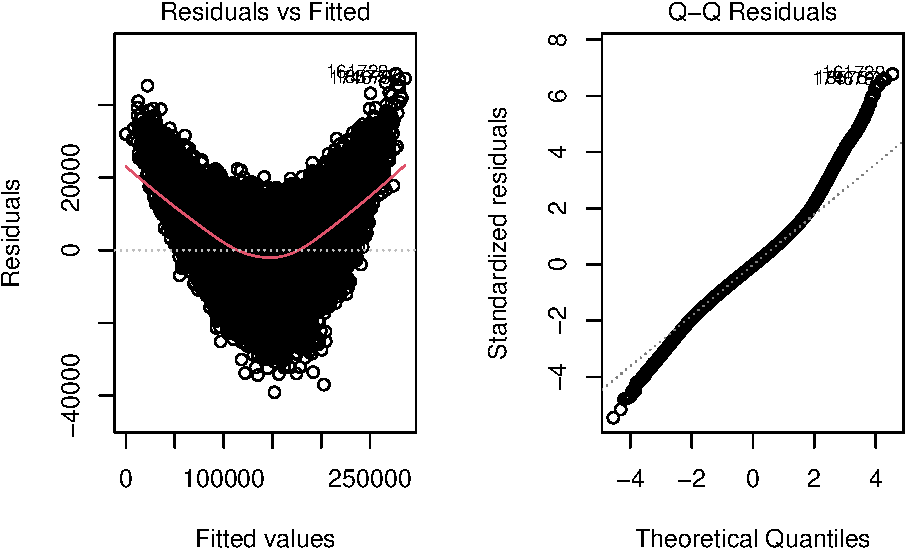
\includegraphics[width=0.8\linewidth,height=0.35\textheight]{INFO248-project2ms1-Wong-Wu_files/figure-latex/unnamed-chunk-21-1} 

}

\caption{Residuals vs. fitted values and Q-Q plot for Model 1.}\label{fig:unnamed-chunk-21}
\end{figure}

The residuals vs.~fitted plot shows a U-shaped curve rather than a
random scatter around zero. The model tends to underpredict salaries at
the low and high ends of the fitted range and slightly overpredict in
the middle. This suggests the relationship between some predictors and
salary is not purely linear. In particular, the effect of experience
years on salary likely follows a curve, with larger gains at earlier
career stages that level off over time. A linear model cannot capture
this shape, so the pattern appears in the residuals. This is a known
limitation of linear regression when predictor effects are non-linear,
and it motivates the use of a more flexible model such as the random
forest in Model 2.

\begin{longtable}[]{@{}
  >{\raggedright\arraybackslash}p{(\linewidth - 8\tabcolsep) * \real{0.3375}}
  >{\raggedleft\arraybackslash}p{(\linewidth - 8\tabcolsep) * \real{0.1625}}
  >{\raggedleft\arraybackslash}p{(\linewidth - 8\tabcolsep) * \real{0.1375}}
  >{\raggedleft\arraybackslash}p{(\linewidth - 8\tabcolsep) * \real{0.1250}}
  >{\raggedleft\arraybackslash}p{(\linewidth - 8\tabcolsep) * \real{0.2375}}@{}}
\caption{Heteroskedasticity-robust (HC3) standard errors for Model
1.}\tabularnewline
\toprule\noalign{}
\begin{minipage}[b]{\linewidth}\raggedright
\end{minipage} & \begin{minipage}[b]{\linewidth}\raggedleft
Estimate
\end{minipage} & \begin{minipage}[b]{\linewidth}\raggedleft
Std. Error
\end{minipage} & \begin{minipage}[b]{\linewidth}\raggedleft
t value
\end{minipage} & \begin{minipage}[b]{\linewidth}\raggedleft
Pr(\textgreater\textbar t\textbar)
\end{minipage} \\
\midrule\noalign{}
\endfirsthead
\toprule\noalign{}
\begin{minipage}[b]{\linewidth}\raggedright
\end{minipage} & \begin{minipage}[b]{\linewidth}\raggedleft
Estimate
\end{minipage} & \begin{minipage}[b]{\linewidth}\raggedleft
Std. Error
\end{minipage} & \begin{minipage}[b]{\linewidth}\raggedleft
t value
\end{minipage} & \begin{minipage}[b]{\linewidth}\raggedleft
Pr(\textgreater\textbar t\textbar)
\end{minipage} \\
\midrule\noalign{}
\endhead
\bottomrule\noalign{}
\endlastfoot
(Intercept) & -181568.9293 & 10173.7067 & -17.8469 & 0.0000 \\
job\_title & 1.0051 & 0.0012 & 828.7222 & 0.0000 \\
experience\_years & 2698.0305 & 2.9145 & 925.7153 & 0.0000 \\
education\_levelDiploma & -5287.5279 & 50.6627 & -104.3672 & 0.0000 \\
education\_levelHigh School & -10664.3465 & 51.4060 & -207.4535 &
0.0000 \\
education\_levelMaster & 10806.0616 & 50.7940 & 212.7427 & 0.0000 \\
education\_levelPhD & 21581.1334 & 53.4270 & 403.9368 & 0.0000 \\
skills\_count & 860.1076 & 3.0392 & 283.0070 & 0.0000 \\
industry & 0.1010 & 0.0698 & 1.4475 & 0.1478 \\
company\_sizeLarge & -14131.9346 & 56.5905 & -249.7227 & 0.0000 \\
company\_sizeMedium & -28311.9427 & 55.1601 & -513.2685 & 0.0000 \\
company\_sizeSmall & -35399.1260 & 56.1612 & -630.3128 & 0.0000 \\
company\_sizeStartup & -42390.3793 & 58.7321 & -721.7588 & 0.0000 \\
location & 0.9980 & 0.0011 & 926.9299 & 0.0000 \\
remote\_workNo & 19.3789 & 40.4162 & 0.4795 & 0.6316 \\
remote\_workYes & 5351.1399 & 40.7605 & 131.2824 & 0.0000 \\
certifications & 1614.6015 & 9.7165 & 166.1704 & 0.0000 \\
\end{longtable}

\begin{longtable}[]{@{}rrl@{}}
\caption{Breusch-Pagan test results for Model 1.}\tabularnewline
\toprule\noalign{}
BP Statistic & df & p-value \\
\midrule\noalign{}
\endfirsthead
\toprule\noalign{}
BP Statistic & df & p-value \\
\midrule\noalign{}
\endhead
\bottomrule\noalign{}
\endlastfoot
5340.521 & 16 & \textless{} 0.0001 \\
\end{longtable}

The Breusch-Pagan test returned a highly significant result, indicating
the presence of heteroskedasticity. However, after applying HC3 robust
standard errors, the significance levels of all predictors were
unchanged, confirming that the coefficient estimates remain reliable
despite the heteroskedasticity.

\subsection{Model 2}\label{model-2}

\begin{longtable}[]{@{}rlr@{}}
\caption{Predictor importance for Model 2 (random forest), ranked by
percent increase in mean squared error.}\tabularnewline
\toprule\noalign{}
Rank & Predictor & \% Increase in MSE \\
\midrule\noalign{}
\endfirsthead
\toprule\noalign{}
Rank & Predictor & \% Increase in MSE \\
\midrule\noalign{}
\endhead
\bottomrule\noalign{}
\endlastfoot
1 & experience\_years & 482.89 \\
2 & company\_size & 425.21 \\
3 & education\_level & 320.58 \\
4 & location & 231.22 \\
5 & job\_title & 171.58 \\
6 & skills\_count & 69.00 \\
7 & certifications & 22.29 \\
8 & remote\_work & 21.24 \\
9 & industry & -0.08 \\
\end{longtable}

These results partially contradict the hypothesis. While location and
job title remain meaningful predictors, experience years, company size,
and education level all ranked above them, suggesting personal factors
carry more salary signal than predicted when non-linear effects are
accounted for.

\begin{figure}

{\centering 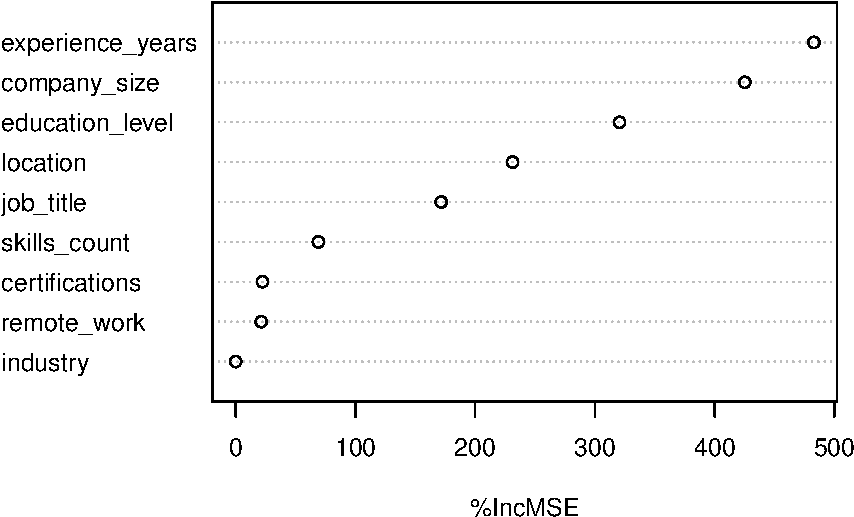
\includegraphics[width=0.7\linewidth,height=0.35\textheight]{INFO248-project2ms1-Wong-Wu_files/figure-latex/unnamed-chunk-26-1} 

}

\caption{Predictor importance plot for Model 2 (random forest).}\label{fig:unnamed-chunk-26}
\end{figure}

This differs from Model 1, where the encoded value tables showed a
\$53,000 salary range across job titles and an \$84,000 range across
locations, suggesting strong job-based salary signals despite their low
coefficient ranks.

Industry ranked last with a negative importance value of -0.08, meaning
removing it from the model would not meaningfully change prediction
accuracy. This is consistent with Model 1's finding that industry
contributes almost no salary signal in this data.

\subsubsection{Model 2 Fit}\label{model-2-fit}

Evaluated on the test set, the random forest produced a root mean
squared error (RMSE) of 12,224 and a mean absolute error (MAE) of 9,812.

\begin{figure}

{\centering 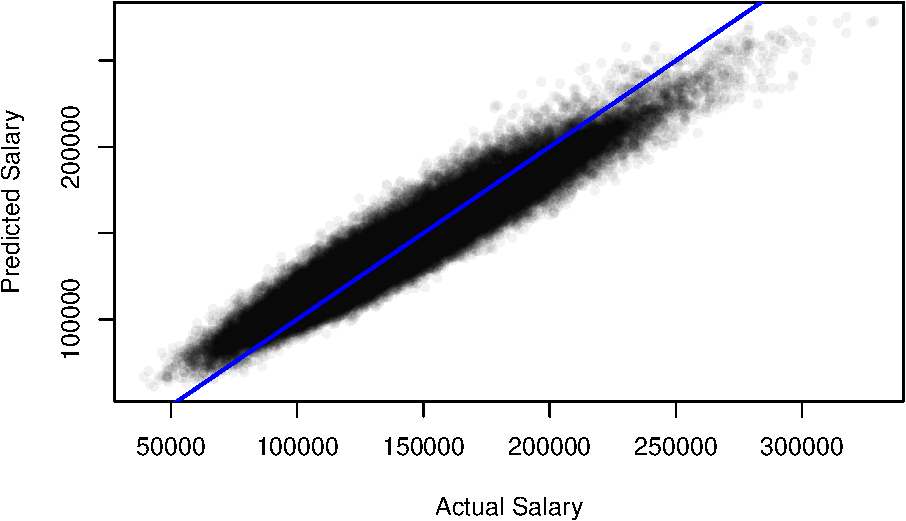
\includegraphics[width=0.7\linewidth,height=0.35\textheight]{INFO248-project2ms1-Wong-Wu_files/figure-latex/unnamed-chunk-28-1} 

}

\caption{Predicted vs. actual salary for Model 2 (random forest) on the test set.}\label{fig:unnamed-chunk-28}
\end{figure}

The predicted vs.~actual salary plot in figure 6 shows the predictions
tracking closely along the diagonal, indicating the model is making
accurate salary estimates across the full range of the outcome. There is
slightly more spread at the higher salary values, suggesting the model
has more difficulty predicting the largest salaries precisely.

\subsection{Comparison of Models 1 and
2}\label{comparison-of-models-1-and-2}

\begin{longtable}[]{@{}lrr@{}}
\caption{Test-set prediction error comparison for Models 1 and
2.}\tabularnewline
\toprule\noalign{}
Model & RMSE & MAE \\
\midrule\noalign{}
\endfirsthead
\toprule\noalign{}
Model & RMSE & MAE \\
\midrule\noalign{}
\endhead
\bottomrule\noalign{}
\endlastfoot
Model 1: Linear Regression & 7122 & 5446 \\
Model 2: Random Forest & 12224 & 9812 \\
\end{longtable}

Model 1 has a lower RMSE than Model 2, which is somewhat surprising
given that random forests are generally more flexible. The likely
explanation is each predictor contributes independently to salary, which
is exactly the structure linear regression is designed for. The target
encoding in Model 1 also gave the linear model an efficient way to
capture the salary signal in high-cardinality categoricals, leveling the
playing field. It should be noted that this comparison is not fully
fair. The random forest, trained on only 10\% of the available data due
to computational constraints, did not have access to the full signal
that the linear model used.

Taking both models together, the hypothesis is partially supported: job
title and location carry broad salary ranges, but experience years,
company size, and education level are stronger predictors overall when
non-linear effects are considered.

\subsection{Model Selection}\label{model-selection}

In the initial model, two predictors showed negligible contributions to
salary prediction. Industry ranked last in importance with a coefficient
near zero, and its encoded values fell within a narrow range across all
ten categories. Remote work showed a similarly weak effect --- the
difference in average salary between hybrid and non-remote positions was
under \$40, and the fully remote premium was modest relative to other
predictors. Both predictors were removed and the model was refit on the
remaining eight predictors.

\begin{longtable}[]{@{}
  >{\raggedright\arraybackslash}p{(\linewidth - 8\tabcolsep) * \real{0.3375}}
  >{\raggedleft\arraybackslash}p{(\linewidth - 8\tabcolsep) * \real{0.1625}}
  >{\raggedleft\arraybackslash}p{(\linewidth - 8\tabcolsep) * \real{0.1375}}
  >{\raggedleft\arraybackslash}p{(\linewidth - 8\tabcolsep) * \real{0.1250}}
  >{\raggedleft\arraybackslash}p{(\linewidth - 8\tabcolsep) * \real{0.2375}}@{}}
\caption{Revised Model 1 coefficient estimates, standard errors, and
significance.}\tabularnewline
\toprule\noalign{}
\begin{minipage}[b]{\linewidth}\raggedright
\end{minipage} & \begin{minipage}[b]{\linewidth}\raggedleft
Estimate
\end{minipage} & \begin{minipage}[b]{\linewidth}\raggedleft
Std. Error
\end{minipage} & \begin{minipage}[b]{\linewidth}\raggedleft
t value
\end{minipage} & \begin{minipage}[b]{\linewidth}\raggedleft
Pr(\textgreater\textbar t\textbar)
\end{minipage} \\
\midrule\noalign{}
\endfirsthead
\toprule\noalign{}
\begin{minipage}[b]{\linewidth}\raggedright
\end{minipage} & \begin{minipage}[b]{\linewidth}\raggedleft
Estimate
\end{minipage} & \begin{minipage}[b]{\linewidth}\raggedleft
Std. Error
\end{minipage} & \begin{minipage}[b]{\linewidth}\raggedleft
t value
\end{minipage} & \begin{minipage}[b]{\linewidth}\raggedleft
Pr(\textgreater\textbar t\textbar)
\end{minipage} \\
\midrule\noalign{}
\endhead
\bottomrule\noalign{}
\endlastfoot
(Intercept) & -164924.0637 & 220.8182 & -746.8770 & 0 \\
job\_title & 1.0045 & 0.0012 & 858.3894 & 0 \\
experience\_years & 2697.5105 & 2.8979 & 930.8581 & 0 \\
education\_levelDiploma & -5266.7001 & 55.6010 & -94.7231 & 0 \\
education\_levelHigh School & -10670.8712 & 55.4737 & -192.3592 & 0 \\
education\_levelMaster & 10833.4809 & 55.4972 & 195.2076 & 0 \\
education\_levelPhD & 21592.2159 & 55.5520 & 388.6845 & 0 \\
skills\_count & 859.8620 & 3.2057 & 268.2284 & 0 \\
company\_sizeLarge & -14165.4517 & 55.4621 & -255.4077 & 0 \\
company\_sizeMedium & -28335.5221 & 55.5553 & -510.0419 & 0 \\
company\_sizeSmall & -35415.4285 & 55.4934 & -638.1913 & 0 \\
company\_sizeStartup & -42424.5852 & 55.6746 & -762.0096 & 0 \\
location & 0.9978 & 0.0008 & 1213.2364 & 0 \\
certifications & 1612.9217 & 10.2912 & 156.7287 & 0 \\
\end{longtable}

\newpage

\begin{longtable}[]{@{}
  >{\raggedright\arraybackslash}p{(\linewidth - 6\tabcolsep) * \real{0.3333}}
  >{\raggedleft\arraybackslash}p{(\linewidth - 6\tabcolsep) * \real{0.0617}}
  >{\raggedright\arraybackslash}p{(\linewidth - 6\tabcolsep) * \real{0.4568}}
  >{\raggedleft\arraybackslash}p{(\linewidth - 6\tabcolsep) * \real{0.1481}}@{}}
\caption{Predictors ranked by importance for the revised Model
1.}\tabularnewline
\toprule\noalign{}
\begin{minipage}[b]{\linewidth}\raggedright
\end{minipage} & \begin{minipage}[b]{\linewidth}\raggedleft
Rank
\end{minipage} & \begin{minipage}[b]{\linewidth}\raggedright
Predictor
\end{minipage} & \begin{minipage}[b]{\linewidth}\raggedleft
Coefficient
\end{minipage} \\
\midrule\noalign{}
\endfirsthead
\toprule\noalign{}
\begin{minipage}[b]{\linewidth}\raggedright
\end{minipage} & \begin{minipage}[b]{\linewidth}\raggedleft
Rank
\end{minipage} & \begin{minipage}[b]{\linewidth}\raggedright
Predictor
\end{minipage} & \begin{minipage}[b]{\linewidth}\raggedleft
Coefficient
\end{minipage} \\
\midrule\noalign{}
\endhead
\bottomrule\noalign{}
\endlastfoot
company\_sizeStartup & 1 & Company Size: Startup vs.~Enterprise &
-42424.59 \\
company\_sizeSmall & 2 & Company Size: Small vs.~Enterprise &
-35415.43 \\
company\_sizeMedium & 3 & Company Size: Medium vs.~Enterprise &
-28335.52 \\
education\_levelPhD & 4 & Education: PhD vs.~Bachelor & 21592.22 \\
company\_sizeLarge & 5 & Company Size: Large vs.~Enterprise &
-14165.45 \\
education\_levelMaster & 6 & Education: Master vs.~Bachelor &
10833.48 \\
education\_levelHigh School & 7 & Education: High School vs.~Bachelor &
-10670.87 \\
education\_levelDiploma & 8 & Education: Diploma vs.~Bachelor &
-5266.70 \\
experience\_years & 9 & Years of Experience & 2697.51 \\
certifications & 10 & Certifications & 1612.92 \\
skills\_count & 11 & Skills Count & 859.86 \\
job\_title & 12 & Job Title (target encoded) & 1.00 \\
location & 13 & Location (target encoded) & 1.00 \\
\end{longtable}

The revised model produced an adjusted R-squared of 0.9635, compared to
0.9633 in the original model, which is a negligible difference
confirming that neither removed predictor was contributing meaningful
predictive power. The test-set RMSE of 7,157 was effectively identical
to the original model.

The importance rankings were stable after removal. The same predictors
that dominated in the original model continued to show the largest
effects, and the encoded value ranges for job title and location
remained unchanged, continuing to support the hypothesis that job-based
factors carry significant salary signal.

\section{Model Prediction}\label{model-prediction}

\textless\textless\textless\textless\textless\textless\textless{} HEAD
We are using repeated cross validation to3 do the model prediction. In
this model, there are 10 folds repeated 3 times with 80\% of the data
used for training on each fold. The first model is linear regression,
while another model is random forest. Due to the large amount of data,
we are randomly select 10\% of the sample for our analysis.

The two tables below shows the training results regarding Linear
Regression and Random Forest model

\subsection{Model 1 Prediction}\label{model-1-prediction}

\begin{longtable}[]{@{}lrrrrrr@{}}
\caption{Model 1 Training Results}\tabularnewline
\toprule\noalign{}
intercept & RMSE & Rsquared & MAE & RMSESD & RsquaredSD & MAESD \\
\midrule\noalign{}
\endfirsthead
\toprule\noalign{}
intercept & RMSE & Rsquared & MAE & RMSESD & RsquaredSD & MAESD \\
\midrule\noalign{}
\endhead
\bottomrule\noalign{}
\endlastfoot
TRUE & 7183.75 & 0.96 & 5462.8 & 155.02 & 0 & 102.34 \\
\end{longtable}

=======

To evaluate how well each model generalizes to unseen data, we used
repeated cross-validation with 10 folds repeated 3 times. In each fold
the data is splt so that 80\% of the data was used ofr training on each
fold and the remaining 20\% held out for testing This process produces
30 total evaluations, and the RMSE and standard deviation are averaged
out across all folds to give a stable estimate of out-of-sample error.

\subsection{Model 1 Prediction}\label{model-1-prediction-1}

\begin{longtable}[]{@{}lrrrr@{}}
\caption{Repeated 10-fold CV results for the linear regression
model.}\tabularnewline
\toprule\noalign{}
Model & Mean RMSE & SD RMSE & Mean MAE & Mean R² \\
\midrule\noalign{}
\endfirsthead
\toprule\noalign{}
Model & Mean RMSE & SD RMSE & Mean MAE & Mean R² \\
\midrule\noalign{}
\endhead
\bottomrule\noalign{}
\endlastfoot
Linear Regression & 7604.59 & 43.25 & 5869.26 & 0.9588 \\
\end{longtable}

\begin{quote}
\begin{quote}
\begin{quote}
\begin{quote}
\begin{quote}
\begin{quote}
\begin{quote}
89e7d69a35337171419fc887901641513f605478
\end{quote}
\end{quote}
\end{quote}
\end{quote}
\end{quote}
\end{quote}
\end{quote}

The linear regression model produced consistent RMSE values across all
30 folds, with a low standard deviation indicating stable
generalization. The mean R-squared is consistent with the adjusted
R-squared reported during model fitting, confirming the model is not
overfitting to the training data.

\subsection{Model 2 Prediction}\label{model-2-prediction}

\textless\textless\textless\textless\textless\textless\textless{} HEAD

\begin{longtable}[]{@{}
  >{\raggedleft\arraybackslash}p{(\linewidth - 16\tabcolsep) * \real{0.0649}}
  >{\raggedleft\arraybackslash}p{(\linewidth - 16\tabcolsep) * \real{0.1818}}
  >{\raggedright\arraybackslash}p{(\linewidth - 16\tabcolsep) * \real{0.1299}}
  >{\raggedleft\arraybackslash}p{(\linewidth - 16\tabcolsep) * \real{0.0779}}
  >{\raggedleft\arraybackslash}p{(\linewidth - 16\tabcolsep) * \real{0.1169}}
  >{\raggedleft\arraybackslash}p{(\linewidth - 16\tabcolsep) * \real{0.1039}}
  >{\raggedleft\arraybackslash}p{(\linewidth - 16\tabcolsep) * \real{0.0909}}
  >{\raggedleft\arraybackslash}p{(\linewidth - 16\tabcolsep) * \real{0.1429}}
  >{\raggedleft\arraybackslash}p{(\linewidth - 16\tabcolsep) * \real{0.0909}}@{}}
\caption{Model 2 Training Results}\tabularnewline
\toprule\noalign{}
\begin{minipage}[b]{\linewidth}\raggedleft
mtry
\end{minipage} & \begin{minipage}[b]{\linewidth}\raggedleft
min.node.size
\end{minipage} & \begin{minipage}[b]{\linewidth}\raggedright
splitrule
\end{minipage} & \begin{minipage}[b]{\linewidth}\raggedleft
RMSE
\end{minipage} & \begin{minipage}[b]{\linewidth}\raggedleft
Rsquared
\end{minipage} & \begin{minipage}[b]{\linewidth}\raggedleft
MAE
\end{minipage} & \begin{minipage}[b]{\linewidth}\raggedleft
RMSESD
\end{minipage} & \begin{minipage}[b]{\linewidth}\raggedleft
RsquaredSD
\end{minipage} & \begin{minipage}[b]{\linewidth}\raggedleft
MAESD
\end{minipage} \\
\midrule\noalign{}
\endfirsthead
\toprule\noalign{}
\begin{minipage}[b]{\linewidth}\raggedleft
mtry
\end{minipage} & \begin{minipage}[b]{\linewidth}\raggedleft
min.node.size
\end{minipage} & \begin{minipage}[b]{\linewidth}\raggedright
splitrule
\end{minipage} & \begin{minipage}[b]{\linewidth}\raggedleft
RMSE
\end{minipage} & \begin{minipage}[b]{\linewidth}\raggedleft
Rsquared
\end{minipage} & \begin{minipage}[b]{\linewidth}\raggedleft
MAE
\end{minipage} & \begin{minipage}[b]{\linewidth}\raggedleft
RMSESD
\end{minipage} & \begin{minipage}[b]{\linewidth}\raggedleft
RsquaredSD
\end{minipage} & \begin{minipage}[b]{\linewidth}\raggedleft
MAESD
\end{minipage} \\
\midrule\noalign{}
\endhead
\bottomrule\noalign{}
\endlastfoot
14 & 5 & variance & 10977 & 0.92 & 8377.59 & 229.43 & 0 & 163.65 \\
\end{longtable}

\begin{longtable}[]{@{}lrrrr@{}}
\caption{Repeated 10-fold CV results for the random forest
model.}\tabularnewline
\toprule\noalign{}
Model & Mean RMSE & SD RMSE & Mean MAE & Mean R² \\
\midrule\noalign{}
\endfirsthead
\toprule\noalign{}
Model & Mean RMSE & SD RMSE & Mean MAE & Mean R² \\
\midrule\noalign{}
\endhead
\bottomrule\noalign{}
\endlastfoot
Random Forest & 16347.66 & 314.88 & 12794.2 & 0.9261 \\
\end{longtable}

The random forest was evaluated on a 10\% sample of the training data
due to computational constraints. The mean RMSE is higher than the
linear regression, and the larger standard deviation across folds
reflects greater variability, likely a result of the reduced training
sample rather than a fundamental weakness of the model.

\begin{longtable}[]{@{}lrrrr@{}}
\caption{Cross-validation performance comparison for both
models.}\tabularnewline
\toprule\noalign{}
Model & Mean RMSE & SD RMSE & Mean MAE & Mean R² \\
\midrule\noalign{}
\endfirsthead
\toprule\noalign{}
Model & Mean RMSE & SD RMSE & Mean MAE & Mean R² \\
\midrule\noalign{}
\endhead
\bottomrule\noalign{}
\endlastfoot
Linear Regression & 7604.59 & 43.25 & 5869.26 & 0.9588 \\
Random Forest & 16347.66 & 314.88 & 12794.20 & 0.9261 \\
\end{longtable}

\subsection{Model Comparison}\label{model-comparison}

\textless\textless\textless\textless\textless\textless\textless{} HEAD
The table below shows the five-number summaries of RMSE in both models.
It clearly illustrates that Random forest has a higher RMSE in
comparison with Linear regression.

\begin{longtable}[]{@{}
  >{\raggedright\arraybackslash}p{(\linewidth - 12\tabcolsep) * \real{0.2308}}
  >{\raggedleft\arraybackslash}p{(\linewidth - 12\tabcolsep) * \real{0.1282}}
  >{\raggedleft\arraybackslash}p{(\linewidth - 12\tabcolsep) * \real{0.1282}}
  >{\raggedleft\arraybackslash}p{(\linewidth - 12\tabcolsep) * \real{0.1282}}
  >{\raggedleft\arraybackslash}p{(\linewidth - 12\tabcolsep) * \real{0.1282}}
  >{\raggedleft\arraybackslash}p{(\linewidth - 12\tabcolsep) * \real{0.1282}}
  >{\raggedleft\arraybackslash}p{(\linewidth - 12\tabcolsep) * \real{0.1282}}@{}}
\caption{Comparison of RMSE Distribution}\tabularnewline
\toprule\noalign{}
\begin{minipage}[b]{\linewidth}\raggedright
\end{minipage} & \begin{minipage}[b]{\linewidth}\raggedleft
Min.
\end{minipage} & \begin{minipage}[b]{\linewidth}\raggedleft
1st Qu.
\end{minipage} & \begin{minipage}[b]{\linewidth}\raggedleft
Median
\end{minipage} & \begin{minipage}[b]{\linewidth}\raggedleft
Mean
\end{minipage} & \begin{minipage}[b]{\linewidth}\raggedleft
3rd Qu.
\end{minipage} & \begin{minipage}[b]{\linewidth}\raggedleft
Max.
\end{minipage} \\
\midrule\noalign{}
\endfirsthead
\toprule\noalign{}
\begin{minipage}[b]{\linewidth}\raggedright
\end{minipage} & \begin{minipage}[b]{\linewidth}\raggedleft
Min.
\end{minipage} & \begin{minipage}[b]{\linewidth}\raggedleft
1st Qu.
\end{minipage} & \begin{minipage}[b]{\linewidth}\raggedleft
Median
\end{minipage} & \begin{minipage}[b]{\linewidth}\raggedleft
Mean
\end{minipage} & \begin{minipage}[b]{\linewidth}\raggedleft
3rd Qu.
\end{minipage} & \begin{minipage}[b]{\linewidth}\raggedleft
Max.
\end{minipage} \\
\midrule\noalign{}
\endhead
\bottomrule\noalign{}
\endlastfoot
Linear\_Regression & 6,822.43 & 7,111.09 & 7,184.94 & 7,183.75 &
7,262.26 & 7,442.16 \\
Random\_Forest & 10,359.54 & 10,861.06 & 10,962.49 & 10,977.00 &
11,124.36 & 11,330.04 \\
\end{longtable}

The performance comparison highlights a significant advantage for the
Linear Regression model. It achieved a substantially lower Mean RMSE
compared to the Random Forest, indicating much higher predictive
accuracy. Furthermore, the SD\_RMSE and the five-number summary reveal
that Linear Regression is more consistent; its maximum error is still
considerably lower than the Random Forest's minimum error, proving it is
the more stable model for this data set.

\begin{longtable}[]{@{}lrr@{}}
\caption{Final Performance Comparison}\tabularnewline
\toprule\noalign{}
Model & Mean RMSE (Accuracy) & SD RMSE (Stability) \\
\midrule\noalign{}
\endfirsthead
\toprule\noalign{}
Model & Mean RMSE (Accuracy) & SD RMSE (Stability) \\
\midrule\noalign{}
\endhead
\bottomrule\noalign{}
\endlastfoot
Linear Regression & 7,183.75 & 155.02 \\
Random Forest & 10,977.00 & 229.43 \\
\end{longtable}

The following table and plot visualize the predictive performance of
both models compared to actual salaries. On the plot, both the Linear
Regression and Random Forest models track the actual salary trends
closely; however, the Linear model exhibits higher variance in certain
regions, occasionally underestimating the actual values more
significantly than the Random Forest.

\begin{figure}

{\centering \includegraphics[width=0.65\linewidth,height=0.28\textheight]{INFO248-project2ms1-Wong-Wu_files/figure-latex/unnamed-chunk-43-1} 

}

\caption{Salary Prediction Comparison}\label{fig:unnamed-chunk-43}
\end{figure}

Below is the first 10 observations comparison of actual salary and model
predictions

\begin{longtable}[]{@{}lrrrr@{}}
\caption{Comparison of Actual vs.~Predicted Salaries}\tabularnewline
\toprule\noalign{}
Row ID & Actual Salary & Linear Pred & RF Pred & Obs ID \\
\midrule\noalign{}
\endfirsthead
\toprule\noalign{}
Row ID & Actual Salary & Linear Pred & RF Pred & Obs ID \\
\midrule\noalign{}
\endhead
\bottomrule\noalign{}
\endlastfoot
57528 & 124,203 & 113,431.84 & 121,420.95 & 1 \\
122496 & 161,207 & 158,600.06 & 160,049.62 & 2 \\
73341 & 141,726 & 150,272.97 & 139,386.20 & 3 \\
136334 & 164,334 & 174,558.98 & 162,194.23 & 4 \\
114007 & 143,589 & 149,862.85 & 142,756.60 & 5 \\
150370 & 170,005 & 163,726.63 & 167,166.74 & 6 \\
159558 & 192,257 & 187,800.30 & 190,329.41 & 7 \\
179632 & 192,554 & 183,664.53 & 170,947.17 & 8 \\
23726 & 95,631 & 97,996.63 & 98,017.59 & 9 \\
114614 & 161,110 & 168,202.53 & 161,757.44 & 10 \\
\end{longtable}

=======

\begin{figure}

{\centering \includegraphics[width=0.7\linewidth,height=0.35\textheight]{INFO248-project2ms1-Wong-Wu_files/figure-latex/unnamed-chunk-45-1} 

}

\caption{RMSE per fold across repeated CV for both models.}\label{fig:unnamed-chunk-45}
\end{figure}

The line plot shows the RMSE across all 30 folds for both models. The
linear regression line remains flat and consistent, confirming stable
generalization across different subsets of the data. The random forest
shows more inconsistent variation, consistent with the higher standard
deviation reported in the table. Overall, the linear regression
outperforms the random forest under cross-validation, which mirrors the
test-set findings reported earlier.

\section{References}\label{references}

{[}1{]}
\url{https://www.kaggle.com/datasets/nalisha/job-salary-prediction-dataset}

\end{document}
